\documentclass[12pt]{report}
\usepackage[utf8]{inputenc}
\usepackage[T1]{fontenc}
\usepackage{mathptmx} % Times body (Phase-2 Letter/Times switch, G-Q6)
\usepackage[scaled=0.92]{helvet} % Arial-like sans for headings
\usepackage{graphicx}
\usepackage{xcolor}
\definecolor{frontpagebg}{RGB}{246,232,177} % sampled from frontpage-color.png
\usepackage{booktabs}
\usepackage{array}
\usepackage{enumitem}
\usepackage{float}
\usepackage{caption}
\usepackage{subcaption}
\usepackage{amsmath}
\usepackage{amssymb}
\usepackage{tikz}
\usetikzlibrary{arrows.meta, positioning, calc, shapes.geometric}
\usepackage{pgfplots}
\pgfplotsset{compat=1.18}
\usepgfplotslibrary{fillbetween}
\usepackage{listings}
\lstset{basicstyle=\ttfamily\footnotesize, breaklines=true, frame=single, showstringspaces=false,
        columns=fullflexible, keepspaces=true, aboveskip=6pt, belowskip=4pt}
\usepackage{titlesec} % Arial Bold headings (Phase-2 Letter/Times switch, G-Q6)
\titleformat{\chapter}[display]{\normalfont\sffamily\bfseries\huge}{\chaptertitlename\ \thechapter}{20pt}{\Huge}
\titleformat{\section}{\normalfont\sffamily\bfseries\Large}{\thesection}{1em}{}
\titleformat{\subsection}{\normalfont\sffamily\bfseries\large}{\thesubsection}{1em}{}
\usepackage[hidelinks]{hyperref}
\usepackage{fancyhdr}
\usepackage{geometry}
\geometry{letterpaper, margin=1in}
\setcounter{secnumdepth}{3} % number sub-subsections (e.g. 2.1.1)

% =====================================================================
% Phase-2 dissertation (full report: Phase-I recap + Phase-II focus).
% MODULAR layout: front matter and bibliography live here; each chapter
% is its own file under chapters/ (edit those). Voice per
% college/mydeliverables/REPORT_WRITING_GUIDE.md (STE-flavored + humanizer
% on body prose only, G1). Figures per TIKZ_DIAGRAM_GUIDE.md.
% Build in /tmp (repo mount is create-only).
% =====================================================================

\begin{document}

\pagecolor{frontpagebg}
\thispagestyle{empty}
\begin{tikzpicture}[remember picture, overlay]
\draw[line width=3pt] ($(current page.north west)+(0.5in,-0.5in)$) rectangle ($(current page.south east)+(-0.5in,0.5in)$);
\end{tikzpicture}
\vspace*{\fill}
\begin{center}

\includegraphics[width=3.5cm]{PESU-new-logo.png} \\[0.3cm]
\textbf{\large Dissertation on}\\[0.3cm]
\textbf{\LARGE ``Adaptive Study Planning for\\ Self-Directed Learners''}\\[0.4cm]
{\small Submitted in partial fulfilment of the requirements for the award of degree of}\\[0.4cm]
\textbf{\large Master of Technology in}\\[0.2cm]
\textbf{\large Data Science and Artificial Intelligence}\\[0.3cm]
\textbf{UE20CS972 Project Phase - 2}\\[0.5cm]
\textbf{Submitted by:}\\
\textbf{Rohit Saji}\\
\textbf{PES2PGE24DS201}\\[0.4cm]
Under the guidance of\\
Prof. Ramesh Prakash Guledgudd\\
PES University\\[0.4cm]
May -- October 2026\\[0.4cm]
{\small M.TECH IN DATA SCIENCE AND ARTIFICIAL INTELLIGENCE\\
FACULTY OF ENGINEERING\\
PES UNIVERSITY\\[0.2cm]
(Established under Karnataka Act No. 16 of 2013)\\
Electronic City, Hosur Road, Bengaluru -- 560 100, Karnataka, India}
\end{center}
\vfill
\null

\newpage
\nopagecolor

% ---- Certificate (sample-styled: black border, white page) ----
\begin{tikzpicture}[remember picture, overlay]
\draw[line width=3pt] ($(current page.north west)+(0.5in,-0.5in)$) rectangle ($(current page.south east)+(-0.5in,0.5in)$);
\end{tikzpicture}
\vspace*{\fill}
\begin{center}

\includegraphics[width=3.5cm]{PESU-new-logo.png}\\[0.3cm]
PES UNIVERSITY\\
(Established under Karnataka Act No. 16 of 2013)\\
Electronic City, Hosur Road, Bengaluru -- 560 100, Karnataka, India\\[0.3cm]
FACULTY OF ENGINEERING\\[0.3cm]
\textbf{\Large CERTIFICATE}
\end{center}

\vfill
This is to certify that the dissertation entitled ``Adaptive Study Planning for Self-Directed Learners'' is a bonafide work carried out by \textbf{Rohit Saji (PES2PGE24DS201)} in partial fulfilment for the completion of Project Phase - 2 (UE20CS972) in the Program of Study -- Master of Technology in Data Science and Artificial Intelligence under the rules and regulations of PES University, Bengaluru during the period May 2026 -- October 2026. It is certified that all corrections/suggestions indicated for internal assessment have been incorporated in the report. The dissertation has been approved as it satisfies the academic requirements in respect of project work.

\vfill
\textbf{External Viva}

\vspace{0.2cm}
\noindent
\begin{tabular}{ll}
Name of the Examiners & Signature with Date \\
1. \rule{5cm}{0.4pt} & \rule{5cm}{0.4pt} \\[0.4cm]
2. \rule{5cm}{0.4pt} & \rule{5cm}{0.4pt} \\
\end{tabular}

\vfill
\noindent
\begin{tabular*}{\textwidth}{@{\extracolsep{\fill}}ccc}
Signature & Signature & Signature \\
Prof. Ramesh Prakash Guledgudd & Dr. Sandesh B J & Dr. Keshavan B K \\
PES University & Chairperson & Dean of Faculty \\
\end{tabular*}
\vfill
\null

\newpage

\section*{Declaration}
I hereby declare that the Project Phase - 2 entitled ``Adaptive Study Planning for Self-Directed Learners'' has been carried out under the guidance of Prof. Ramesh Prakash Guledgudd, and submitted in partial fulfilment of the course requirements for the award of the degree of Master of Technology in Data Science and Artificial Intelligence of PES University, Bengaluru, during the academic semester May -- October 2026.

\newpage

\section*{Acknowledgement}
I would like to express my gratitude to my guide for continuous guidance and support throughout this project, and to the project coordinators for their help. I thank the Chairperson and faculty of the Department, PES University, for their support, and the university leadership for the opportunities provided. Finally, I extend heartfelt thanks to my family and friends for their constant encouragement.

\newpage

\section*{Abstract}
Self-directed learners routinely commit to a fixed study plan and fall behind or move ahead within days, yet the plan does not adapt and the learner has no reliable signal of how far off-track they are. Phase~I of this work built an open-loop adaptive planner that estimates the learner's true study pace from session history, detects behavioral shifts in that pace, and projects the completion date with an uncertainty band, regenerating the plan when the projection diverges from the deadline. The open loop adapts to pace but never checks learning: logged hours do not prove that studying produced understanding. Phase~II closes the loop with assessment-based verification of graded evidence. The system generates grounded assessments in three question families from the learner's own materials, grades each family with an authoritative arm, tracks mastery with Bayesian knowledge tracing, guides with a Socratic ladder and a gated reveal, returns advisory feedback copy, runs mixed practice through the library and practice hub, and replans from the loop verdict. Each component is evaluated against baselines and live runs, and the closed loop undergoes integration validation on synthetic longitudinal histories across four learner archetypes, with no fixed-plan control. Learning gain is not measured: the replay covers integration behavior on synthetic histories, and efficacy on learning remains future work. The selected models are realized in a working local-first web application.

\textbf{Keywords:} adaptive study planning, knowledge tracing, grounded generation, rubric grading, learning analytics.

\newpage
\tableofcontents
\newpage
\listoffigures
\newpage
\listoftables
\newpage

% ---- Running header and footer rule (body pages only) ----
\pagestyle{fancy}
\fancyhf{}
\fancyhead[LE,RO]{\small\textit{\leftmark}}
\fancyfoot[C]{\thepage}
\renewcommand{\headrulewidth}{0.4pt}

% ---- Definitions and Abbreviations (Batch 1, R-09) ----
\chapter*{Definitions and Abbreviations}
\addcontentsline{toc}{chapter}{Definitions and Abbreviations}
{\footnotesize
\begin{tabular}{p{3.2cm} p{11.2cm}}
\toprule
\textbf{Term} & \textbf{Meaning in this report} \\
\midrule
AC1--AC4 & Acceptance Criteria 1--4 for the live deployment check (Sec~6.2). \\
S-layer & Generation sweep aggregate (n=180). S:1--S:6 are the six distinct groundedness question keys; S:off is the delivered reasoning-off arm (Sec~6.1). \\
ECE & Expected Calibration Error for mastery tracing (Sec~6.1). \\
ACCA & Frozen ACCA study text: 754 chunks with 768-dimensional sidecar vectors; primary offline corpus (Sec~5.2, 6.1). \\
DDIA & Second corpus: 1094 chunks; confirms the retrieval direction (Sec~5.2, 6.1). \\
OULAD & Open University dataset; calibrates the Phase~I generator only, outside the Phase~II comparison (Sec~5.2). \\
Posture & Planted weekly behavior pattern per synthetic archetype: steady, crammer, struggling, returning (Sec~4.3, 5.2). \\
Sufficiency & Judge evidence-sufficiency score for the loop verdict; converted replans read 0.66--0.77 (Sec~4.1, 6.3). \\
Verdict pair & Exact verdict payload mirrored from \texttt{suggest\_replan} onto \texttt{RoadmapReplanned} (Sec~4.1, 6.3). \\
Dip-window & Week-3 trough replay with the browser clock pinned; trough holds on the merits (Sec~6.4). \\
Met-class & Agreement-met subset in the Jev train/test split; the shipped cutoff rests on two pairs (Sec~6.1). \\
Top-up & Fresh live coding pull after the pre-top-up gold run, which reads 0.0 derivable (Sec~6.1). \\
Gate fix & Loop gate moved from 0.9 to 0.7 (\texttt{LOOP\_APPROVE\_AT} 0.7); confidence 1.0 would also clear the old gate (Sec~4.2.5, 6.3). \\
\bottomrule
\end{tabular}
}

\newpage

% ---- Chapters (modular; one file each under chapters/) ----
\chapter{Introduction}
This chapter sets out the problem this phase addresses and the shape of the work that follows. Section~1.1 recalls the Phase~I system in one paragraph. Section~1.2 states the Phase~II problem. Section~1.3 lists the objectives of Phase~II, each with a short explanation. Section~1.4 defines the scope of the work across both phases. Section~1.5 maps the chapters that follow.

\section{Background}
A self-directed learner is a person who works through online courses, examination preparation, or self-study material without an instructor setting the pace. Such a learner typically begins with a fixed plan, of the form ``two hours a day, finish by this date.'' Within days the plan no longer matches reality, and the fixed finish date quietly turns wrong while the plan still displays it as though it were still valid. Phase~I of this project built an open-loop adaptive planner for this learner. The system estimated true study pace from session history with hierarchical Bayesian calibration, flagged genuine shifts in pace with CUSUM change-point detection, projected the completion date with a calibrated uncertainty band using Gaussian-process regression, and regenerated the schedule from realised capacity when the projection diverged from the deadline. Each component was compared against baselines on a synthetic dataset with known ground truth, using held-out evaluation with bootstrap confidence intervals and multiple-comparison correction, and the selected models were realised in a working local-first web application. The comparison reported its nulls honestly: the calibrated pace beat the fixed-rate baseline only after enough sessions had accumulated, and change detection stayed a documented robust null when no candidate dominated the frontier. What the open-loop system never checked was whether the logged hours produced learning.

\section{Problem Statement}
The pace signal in Phase~I comes from self-reported session logs. It records study time and says nothing about understanding. A learner can log every planned hour and still fail every test, while the plan keeps praising the pace and the examination result collapses. Existing tools leave the same gap open from the other side. Time-tracking applications record hours without judging understanding, and static plan generators never revise against any evidence at all. The missing piece is assessment-based verification of genuine learning, wired into the planning loop so that grades drive the decision to stay the course or replan. Phase~II closes this loop. It generates grounded assessments from the learner's own materials, grades them with an authoritative arm per question family, tracks mastery from the grade history, and feeds a verdict on the plan back into schedule regeneration.

\section{Objectives}
Phase~II of the project pursues the following objectives.
\begin{enumerate}
\item Generate grounded assessments in three families. Each generation call produces one question in a single family, objective, written, or coding, grounded in retrieved chunks of the learner's material with recorded citations. A mixed run alternates the family per call, so every question stays traceable to the material it tests.

\item Grade each family with its authoritative arm. Objective questions grade deterministically against authored answers, written answers grade against a rubric applied by a language model, and coding answers execute in a sandboxed runner with hidden tests. The server grade is authoritative. Any client-side check stays advisory and never reaches the record.

\item Estimate mastery with Bayesian knowledge tracing and steer difficulty from it. A Bayesian model updates a per-skill mastery probability from the graded response history, and the practice system adapts the difficulty of upcoming problems to the estimate instead of serving a fixed sequence.

\item Guide with a Socratic ladder and a gated reveal. The coach answers questions through a ladder of Nudge, Hint, Targeted explanation, and Reveal, and the final step stays locked until the learner confirms. Guidance therefore never hands over the answer before the learner has worked.

\item Return advisory feedback copy on each graded attempt. A server endpoint drafts learner-facing feedback grounded in the attempt and its citations for updated entries, with a static fallback when the model is unreachable. The copy never alters the grade.

\item Run mixed practice through the library and practice hub. Assessments and practice runs live under the material library with cache-first loading, and a practice run resolves its questions lazily from the loaded assessments. Starting practice therefore stays fast even on slow networks.

\item Replan from the loop verdict and validate the loop on synthetic longitudinal histories. A loop endpoint reads mastery, posture, and grade evidence and returns a hold or replan verdict under a fixed confidence gate, and a verdict for replan carries into schedule regeneration with its identity attached. Four synthetic learner archetypes over five weeks each supply the longitudinal histories that a single-semester project cannot collect from real learners.
\end{enumerate}

\section{Scope of the Project}
The work is delivered across two phases. \textbf{Phase~I}, reported earlier, built and evaluated the open-loop system: pace calibration, change detection, completion projection, and capacity-based schedule regeneration, each compared offline against baselines and realised in the application. \textbf{Phase~II}, reported here, closes the loop with assessment-based verification of genuine learning: grounded generation, authoritative grading, mastery tracing, Socratic guidance, advisory feedback, mixed practice runs, and verdict-driven replanning, validated on synthetic longitudinal histories. The target user in both phases is the individual self-directed learner. Multi-user, institutional, and instructor-mediated settings remain out of scope, as does deployment in a real classroom. The synthetic archetypes stand in for the longitudinal real-learner study a single semester cannot supply.

\section{Organization of the Report}
The remainder of the report is organized as follows. Chapter~2 surveys the research this phase draws on: Sections~2.1 to~2.4 cover knowledge tracing, item generation and tagging, grading, and guidance with feedback, Section~2.5 notes the sourcing method, and Section~2.6 summarizes the approaches and the gaps this project addresses. Chapter~3 specifies the system requirements in Sections~3.1 to~3.4. Chapter~4 describes the proposed methodology: the closed loop in Section~4.1, the selected models in Section~4.2, the comparison method in Section~4.3, the design evolution in Section~4.4, and the system architecture in Section~4.5. Chapter~5 gives the implementation details in Sections~5.1 to~5.5. Chapter~6 presents the results and discussion in Sections~6.1 to~6.5. Chapter~7 concludes in Section~7.1 and sets out future work in Section~7.2.

\chapter{Literature Survey}
This chapter surveys the techniques this phase draws on. Section~2.1 covers knowledge tracing and mastery models. Section~2.2 reviews automatic item generation and knowledge-component tagging. Section~2.3 describes grading methods for written and coded answers. Section~2.4 surveys Socratic guidance and learner feedback. Section~2.5 notes the method used to source the surveyed models. Section~2.6 summarizes the approaches and states the gaps this project addresses.
% Drafting starts here (grill pending).

\chapter{System Requirements Specification}
This chapter specifies the requirements of the full system. Sections~3.1 and~3.2 state the hardware and software environment. Section~3.3 lists FR-1 to FR-15, and Section~3.4 lists NFR-1 to NFR-9. FR-9 to FR-15 and NFR-7 to NFR-9 cover the Phase~II additions.

The chapter assumes a single self-directed learner, a workstation with a graphics processor, and access to the hosted model APIs. It also assumes that synthetic longitudinal histories replace a classroom study, as stated in Section~1.4.

\section{Hardware Requirements}
The system runs on a single workstation. A single learner produces a small volume of data with tens to hundreds of sessions. Statistical models train and run on the CPU. Embedding and rerank calls run on the graphics processor, so the workstation includes a discrete graphics processor. Table~\ref{tab:hardware} lists the minimum hardware environment. A note under the table records the project machine.

\begin{table}[htbp]
\centering
\caption{Hardware environment.}
\label{tab:hardware}
\begin{tabular}{p{4.2cm} p{8.0cm}}
\toprule
\textbf{Component} & \textbf{Minimum requirement} \\
\midrule
Processor & x86-64 CPU with a discrete graphics processor \\
Memory & 8~GB RAM or higher \\
Storage & At least 60~GB free for the container images, before build cache and volumes \\
Container runtime & Docker to run the intelligence service, the worker, the GPU inference sidecar, and the sandbox \\
Client device & Any device with a current browser that supports IndexedDB and ES2022 \\
\bottomrule
\end{tabular}
\end{table}

The project machine uses an AMD Radeon RX~9070~XT and has 19~GB of RAM. Its container images measure about 53~GB: 49.5~GB for the GPU sidecar, 1.42~GB for Piston, and about 1.7~GB for the product images. Build cache and volumes bring the total to about 74~GB, and browser data stays within the browser's per-origin quota.

\section{Software Requirements}
The system keeps the Phase~I tiers and adds the GPU inference sidecar plus the code-execution sandbox. The browser client stays local-first. The Python intelligence service and its worker now host generation, grading, mastery, guidance, and feedback. Supabase still provides authentication, the event database, and object storage. The GPU inference sidecar serves embeddings and rerank scores, and the sandbox runs learner code. Table~\ref{tab:software} lists the software environment by tier.

\begin{table}[htbp]
\centering
\caption{Software environment by tier.}
\label{tab:software}
\begin{tabular}{p{3.6cm} p{8.6cm}}
\toprule
\textbf{Tier} & \textbf{Technologies} \\
\midrule
Client (single-page app) & React~19, Vite~5, TypeScript, Dexie over IndexedDB for local-first storage, date-fns \\
Intelligence service and worker & Python~3.12, FastAPI, Uvicorn, NumPy, PyJWT, generation, grading, mastery, guidance, and feedback endpoints, packaged with Docker \\
Model providers & OpenRouter generation and rubric-grading provider (\texttt{deepseek/deepseek-v4-flash-0731}), plus the Jev-1.13 advisory judgment client \\
Backend services & Supabase: authentication, a PostgreSQL event database including \texttt{jev\_review\_flags} for the written-arm review queue, and object storage \\
GPU inference sidecar & Qwen3-Embedding-0.6B plus Qwen3-Reranker-0.6B behind \texttt{/embed} and \texttt{/rerank}, separate compose project \\
Code-execution sandbox & Piston (\texttt{ghcr.io/engineer-man/piston}) on port~2000 for hidden-test grading \\
Offline research pipeline & Python (uv workspace), NumPy, with pytest and ruff for testing and linting \\
Tooling and deployment & pnpm workspace, Vitest and Playwright for testing, Vercel for hosting \\
\bottomrule
\end{tabular}
\end{table}

\section{Functional Requirements}
The functional requirements state what the system does. Items FR-1 to FR-8 carry the Phase~I planner. Items FR-9 to FR-15 add the assessment-verified loop.
\begin{enumerate}[label=\textbf{FR-\arabic*},noitemsep,leftmargin=*]
    \item The system shall let a learner define a study plan from a set of materials, a deadline, and a weekly study capacity.
    \item The system shall log study sessions, both from an in-application timer and from manual entry of a past session.
    \item The system shall estimate the learner's pace from the logged sessions using hierarchical Bayesian calibration.
    \item The system shall detect a shift in the learner's pace and surface a recalibration prompt for the learner to act on.
    \item The system shall project the completion date with an uncertainty band rather than a single date.
    \item The system shall regenerate the schedule from the learner's realized capacity when the learner chooses to replan.
    \item The system shall present the learner's progress, including the burn-up curve, streak, and schedule adherence.
    \item The system shall persist all data on the device and synchronize it to the cloud when a connection is available.
    \item The system shall generate one grounded question per call in a single family, with each question carrying its recorded chunk citations.
    \item The system shall grade each family with its authoritative arm. Deterministic grading applies to objective items. Rubric grading with the OpenRouter rubric model applies to written items. Jev-1.13 is an advisory shadow and the loop-verdict judge. Hidden-test pass rate applies to coding items.
    \item The system shall estimate mastery per skill with the \texttt{bkt-v1} model and provide an advisory difficulty recommendation from that estimate. The recommendation is not calibrated (see Section~6.1).
    \item The system shall guide the learner through a Nudge, Hint, Targeted explanation, and Reveal ladder and keep the full answer gated behind an explicit reveal.
    \item The system shall supply advisory feedback copy on updated results only, and that copy shall never alter a grade.
    \item The system shall run mixed practice sessions through the assessment library and the practice hub, with pause as leave-and-return.
    \item The system shall replan from the loop verdict once assessment evidence shows the plan is off track. Logged hours alone do not trigger a replan (see Section~4.1 for the hold rule and Section~6.3 for the replay evidence).
\end{enumerate}

\section{Non-Functional Requirements}
The non-functional requirements state the qualities the system must exhibit. Items NFR-1 to NFR-6 carry the Phase~I qualities, with NFR-2 restated from the Phase~I CPU-only form to cover the single-GPU sidecar. Items NFR-7 to NFR-9 add the measurable Phase~II qualities.
\begin{enumerate}[label=\textbf{NFR-\arabic*},noitemsep,leftmargin=*]
    \item \textbf{Offline-first operation.} The core logging loop shall function without network connectivity, and analytical results shall be cached locally for reuse.
    \item \textbf{Single-GPU scale.} The system shall serve the individual-learner workload on one workstation graphics processor, with no cluster and no multi-GPU setup.
    \item \textbf{Per-learner isolation.} Each learner's data shall be isolated, using a per-user local database and row-level security in the cloud database.
    \item \textbf{Authenticated services.} Requests to the intelligence service shall carry a signed token that is verified against the identity provider before any model runs.
    \item \textbf{Responsiveness.} Calibration results shall return within 8~s per attempt, with at most two retries, so the worst case is three attempts. Projection runs locally without a network call. The client keeps the last cached result with a stale flag when the service is unreachable.
    \item \textbf{Behavioral alignment.} Where an algorithm exists in both the client and the service, the two implementations shall stay behaviorally aligned on versioned golden fixtures. Calibration and roadmap engines replay the same fixtures in TypeScript and Python with numeric equality to a tight tolerance.
    \item \textbf{Grounded generation.} The judged groundedness of generated questions shall be at least 0.80 on a 30-question sample (the Section~6.1 arm reads 0.8667).
    \item \textbf{Grade authoritativeness.} Hidden tests, reference solutions, and authored accepted values shall never reach the browser, and the server grade shall be final while client results stay advisory.
    \item \textbf{Retrieval quality floor.} Retrieval shall hold recall at 1 of 0.60 and recall at 3 of 0.85. It shall hold a mean reciprocal rank of 0.75 on the frozen ACCA 754-chunk corpus. The floor sits below the \texttt{hybrid\_rerank} arm (0.67, 0.90, 0.797 on n=30, see Section~6.1).
\end{enumerate}
NFR-7 and NFR-9 are prospective floors with headroom below the measured arms, not the measured values themselves.

\section{Product Perspective}
The product is a local-first web application. A TypeScript client with a per-user browser store talks to a Python intelligence service with a portless worker. Supabase is the auth, database, and storage hub. Phase~I delivered the planner substrate of session runtime, progress views, and roadmap lifecycle, and that substrate is unchanged. Phase~II adds assessment generation, per-family grading, mastery tracing, Socratic guidance, advisory feedback, mixed practice, and the loop verdict on top of it.

The only actor is the single self-directed learner. Multi-user, institutional, and instructor-mediated settings are out of scope. External interfaces are the browser, the Supabase project, the OpenRouter API for generation, grading, and judging, and the two sidecars for embeddings and code execution.

\section{Assumptions, Dependencies and Constraints}
The work assumes one learner with their own materials in text, PDF, or web-article form. The learner runs a modern browser with local storage on a steady network for service calls. It depends on a Supabase project for auth, database, and storage. It also needs an OpenRouter key for the generation, grading, and judge models, the Qwen3 sidecar models, and the Piston image for code execution.

Generation and grading call a third party, so learner material leaves the device. The report states no retention contract. The build constrains deployment to a single workstation graphics processor with no cluster. The loop verdict constrains replans to evidence the grades support.. The build constrains deployment to a single workstation graphics processor with no cluster, and the loop verdict constrains replans to evidence the grades support.

\section{Operating Environment}
The stack runs containerized. Web, intelligence, ingestion worker, and Piston form the product compose project. The Qwen3 embedding and rerank sidecar has its own compose project on port~8200. Local development runs the Python 3.12 service on port~8000 and the React client on port~5173. The sandbox profile on port~2000 runs under Docker Desktop on WSL2.

The client needs only a modern browser with IndexedDB. All heavy compute stays server-side or in the sidecars.

\chapter{Proposed Methodology}
This chapter describes how the closed loop works and why it takes this shape. Section~4.1 presents the closed learning loop. Section~4.2 states the candidate models and the selected approach. Section~4.3 describes the comparison methodology. Section~4.4 traces the design evolution. Section~4.5 presents the system architecture.
% Drafting starts here (grill pending).

\chapter{Implementation Details}
This chapter describes how the Phase~II system is built. Sections~5.1 and~5.2 record the development environment and the datasets. Section~5.3 describes the model and service implementation. Section~5.4 records how the metrics are kept reproducible. Section~5.5 presents the Phase~II application.

\section{Development Environment}
The project keeps the Phase~I repository shape. A pnpm workspace holds the TypeScript client with its shared engines. A uv workspace holds the Python packages, the service, and the research code. The two coexist so that the research code imports the same Python engines the service runs.

Table~\ref{tab:tools} lists the environment. The first eleven rows carry the Phase~I stack unchanged. The last seven rows add the Phase~II generation, grading, feedback, judgment, sandbox, embedding, and editor concerns.

\begin{table}[htbp]
\centering
\footnotesize
\caption{Development environment: tools and libraries. The first eleven rows carry the Phase~I stack; the last seven add the Phase~II loop.}
\label{tab:tools}
\begin{tabular}{p{4.0cm} p{8.4cm}}
\toprule
\textbf{Concern} & \textbf{Technology} \\
\midrule
Client language and build & TypeScript, Vite, pnpm workspace \\
Client UI & React~19 \\
Local-first storage & Dexie over IndexedDB \\
Intelligence service & Python~3.12, FastAPI, Uvicorn \\
Scientific stack & NumPy, SciPy \\
Service authentication & PyJWT, verifying Supabase-issued tokens \\
Containerisation & Docker Desktop on WSL2 (Compose) \\
Python workspace & uv \\
JavaScript testing & Vitest, fast-check (property tests), Playwright (end-to-end) \\
Python testing and linting & pytest, ruff \\
Backend and hosting & Supabase (auth, database, storage), Vercel \\
Generation provider & OpenRouter, \texttt{deepseek/deepseek-v4-flash-0731}, temperature 0.3, reasoning off, 30~s timeout \\
Rubric-grading model & \texttt{deepseek/deepseek-v4-flash-0731} through \texttt{GRADING\_MODEL}, the authoritative written-arm score \\
Feedback-copy model & \texttt{meta/muse-spark-1.3-contributor} through \texttt{FEEDBACK\_MODEL}, reasoning effort low \\
Judgment client & Jev-1.13 hosted System One API through \texttt{OPENROUTER\_JEV\_API\_KEY}, advisory shadow and loop-verdict judge \\
Code-execution sandbox & Piston sandbox profile on port~2000 for hidden-test grading \\
 GPU inference sidecar & Qwen3-Embedding-0.6B and Qwen3-Reranker-0.6B on port~8200 in a separate compose project \\
Client code editor & CodeMirror with an advisory Pyodide check that never grades \\
\bottomrule
\end{tabular}
\end{table}

\section{Datasets and Their Sources}
A single learner's real log does not supply a known ground truth for latent mastery and pace in this design. The Chapter~6 comparison therefore runs on fixed artifacts with planted and known properties. Table~\ref{tab:datasets} lists the datasets and the role each plays.

The frozen corpus is a single textbook (edition needs verification) at 754 chunks with 768-dimensional sidecar vectors. Three gold files score the offline leg against it: the objective probe set, the written gold set, and the coding gold set. The fixed folds and the attempt gate sit beside them in \texttt{eval\_golds.json}.

The longitudinal leg replays four synthetic archetypes with known posture: steady, crammer, struggling, and returning. Their generator plants weekly pace, skip behavior, gap weeks, and replan back-pointers explicitly. The Open University dataset (version needs verification) calibrates the Phase~I generator only and does not enter the Phase~II comparison. Real single-learner logs stay reserved for future validation and are not used here.

\begin{table}[htbp]
\centering
\footnotesize
\caption{Datasets used in Phase~II and their sources.}
\label{tab:datasets}
\begin{tabular}{p{3.6cm} p{3.8cm} p{5.0cm}}
\toprule
\textbf{Dataset} & \textbf{Source} & \textbf{Role} \\
\midrule
 Frozen corpus and harness golds & In-repository gold files: \texttt{eval\_golds.json} with probe, written, and coding sets. ACCA text at 754 chunks with 768-dimensional sidecar vectors (edition needs verification) & Primary ground truth for the offline leg: generation, retrieval, mastery, and coding checks \\
 Synthetic longitudinal histories & In-repository generator with four archetypes: steady, crammer, struggling, and returning & Whole-loop replay with known posture, and the post-fix replay evidence is versioned \\
 OULAD & Public Open University dataset (version needs verification) & Calibration source for the Phase~I generator \\
 Real session logs & The candidate's own sessions & Reserved for future validation, outside the Phase~II comparison \\
\bottomrule
\end{tabular}
\end{table}

\section{Model and Service Implementation}
Each algorithm has one behavioral definition. The client and service hold separate implementations only where the client must compute a view locally. The client-side engines are written in TypeScript, and a Python mirror of each engine runs behind the intelligence service. A golden-fixture parity harness keeps the two implementations aligned.

The TypeScript engines emit reference inputs and outputs. A Python test replays each input and asserts numeric equality within a 1e-6 relative and absolute tolerance. The shared numeric constants, such as the BKT parameters, stay identical on both sides.

The split between client and service follows the architecture of Figure~\ref{fig:architecture}. Service-side code owns grounded generation, per-family grading arms, and the mastery endpoint. It also owns the guide stream with its gated reveal. It further owns the feedback-copy endpoint and the loop verdict with the Jev judge as a hosted-API client. The client keeps the engines it must read locally. Those are the roadmap bookings, the Gaussian-process projection, the mastery readers with the difficulty chip, and the verdict handoff.

The offline research harness imports the production Python engines as candidates. It never re-implements them, so an offline result measures the same engine code the service runs. Listing~\ref{lst:bktforward} shows the shipped BKT forward filter, which realizes Equation~\ref{eq:bkt-update}, and Table~\ref{tab:packages} lists the main packages.

\noindent\begin{minipage}{\linewidth}
\begin{lstlisting}[language=Python, caption={The shipped BKT forward filter, which realizes Equation~\eqref{eq:bkt-update}.}, label={lst:bktforward}]
def bkt_forward(
    observations: list[MasteryObservation],
    params: BktParams = DEFAULT_PARAMS,
) -> tuple[list[float], list[float]]:
    """Run the forward filter over one skill's observation sequence.

    Returns ``(mastery_after, p_correct_before)`` parallel lists:
    ``p_correct_before[i]`` is the predicted probability of correctness for
    observation ``i`` computed from the belief before it, and
    ``mastery_after[i]`` is P(mastery) after processing observation ``i``.
    """

    mastery: list[float] = []
    p_correct: list[float] = []
    belief = params.p_init
    for obs in observations:
        p_correct.append((1.0 - params.p_slip) * belief + params.p_guess * (1.0 - belief))
        if obs.correct:
            numerator = (1.0 - params.p_slip) * belief
            denominator = numerator + params.p_guess * (1.0 - belief)
        else:
            numerator = params.p_slip * belief
            denominator = numerator + (1.0 - params.p_guess) * (1.0 - belief)
        belief = numerator / denominator if denominator > 0 else belief
        belief += (1.0 - belief) * params.p_learn
        mastery.append(float(np.clip(belief, 0.0, 1.0)))
    return mastery, p_correct
\end{lstlisting}
\end{minipage}

\begin{table}[H]
\centering
\footnotesize
\caption{Main packages and their roles.}
\label{tab:packages}
\begin{tabular}{p{4.8cm} p{7.6cm}}
\toprule
\textbf{Package / module} & \textbf{Role} \\
\midrule
\texttt{packages/progress} (TS) & Client mastery engine with bkt-v1: projection and the difficulty chip \\
 \texttt{packages/roadmap-engine} (TS) & Client booking and roadmap generation. The booking model is unchanged \\
\texttt{packages/py-progress} (Py) & Python mirror: Bayesian and enriched-shrinkage calibration, CUSUM, Gaussian process, bkt-v1 \\
\texttt{packages/py-roadmap-engine} (Py) & Python mirror of the roadmap engine \\
\texttt{services/intelligence} (Py) & FastAPI service with a portless worker: generation, grading, mastery, guide, feedback, and the loop verdict \\
\texttt{services/embedder} & Qwen3 embedding and rerank sidecar in a separate compose project \\
Piston sandbox & External image for hidden-test code execution, started on demand \\
 Research scripts & Offline harness and probes, importing the production engines \\
\bottomrule
\end{tabular}
\end{table}

Code answers execute in the self-hosted Piston sandbox through the profile on port~2000. Hidden tests and reference solutions stay server-side. The client runs visible tests only as advice. No resource or egress bound for that sandbox is stated in this report (see Section~6.6).

Table~\ref{tab:phase2-api} lists the Phase~II service surface. Every route verifies the signed Supabase token before any model runs. Every call sends one \texttt{X-Request-ID}, and failures answer with typed service errors that fail closed.

\begin{table}[htbp]
\centering
\footnotesize
\caption{Phase~II service surface: method, auth, contract, and errors.}
\label{tab:phase2-api}
\begin{tabular}{p{4.6cm} p{7.8cm}}
\toprule
\textbf{Route} & \textbf{Contract} \\
\midrule
\texttt{POST} \newline \texttt{/v1/assessments/generate} & One material, one family, one question. Tracked job. Rejects multi-family calls. Terminal states never retry \\
\texttt{POST} \newline \texttt{.../attempts} & One answer per question. Never touches hidden tests or reference solutions \\
\texttt{POST} \newline \texttt{/v1/guide/stream} & Server-sent events with monotonic sequence. Gated Reveal stays locked \\
\texttt{POST} \newline \texttt{/v1/guide/reveal} & Requires confirmation plus the owned attempt bound to the question \\
\texttt{GET} \newline \texttt{/v1/mastery}, \texttt{/recommendations} & Stateless per-skill estimate plus one-band advisory recommendation \\
\texttt{POST} \newline \texttt{/v1/feedback/copy} & Drafts text for updated entries only. Static fallback. Never alters a grade \\
\texttt{POST} \newline \texttt{/v1/loop/decision} & Judge proposes, code router disposes at evidence 0.5 and confidence 0.7 \\
\texttt{POST} \newline \texttt{/v1/retrieval/search} & Owner-scoped chunks. Optional rerank flag with top-k reorder \\
\bottomrule
\end{tabular}
\end{table}

\section{Evaluation Metrics and Reproducibility}
The metrics used to score each loop stage are defined in Table~\ref{tab:phase2-metrics} of Chapter~4. This section records how the project keeps them reproducible.

Three facts carry the reproducibility claim. First, every gate fails closed by default. The evaluation harness stays inert unless the caller passes \texttt{-{}-activate}. The loop router maps a judge failure onto \texttt{hold} through a typed service error. The grading arms return a deterministic fail-closed outcome for unusable input and never fabricate a score.

Second, every call carries one request identifier from the browser to the service logs. The client sends \texttt{X-Request-ID} on each intelligence call. The service echoes it on each response, and every error log line carries it. One identifier therefore joins the frontend, the backend, and the end-to-end evidence.

Third, a reader can re-run both legs from versioned inputs and the documented services. The offline leg needs \texttt{eval\_golds.json} with \texttt{eval\_harness.py} and the documented Supabase, sidecar, and judge access. The longitudinal leg needs the synthetic generator with the four archetypes and the versioned post-fix replay evidence.

Table~\ref{tab:phase2-hyperparams} records the hyperparameters a rerun must hold fixed. Table~\ref{tab:phase2-testing} records the test inventory behind the delivered code. There is no continuous-integration gate: verification is agent-run per the repository workflow, and coverage is not measured.

\begin{table}[htbp]
\centering
\footnotesize
\caption{Hyperparameters a rerun must hold fixed.}
\label{tab:phase2-hyperparams}
\begin{tabular}{p{4.8cm} p{7.6cm}}
\toprule
\textbf{Parameter} & \textbf{Value} \\
\midrule
Chunking & About 400 tokens per chunk with about 30 tokens of overlap \\
Embedding & 768 dimensions from the Qwen3 sidecar \\
Generation retrieval & Top 5 owner-scoped chunks per call \\
Endpoint search & Top 50 candidates before rerank \\
Generation model & Temperature 0.3, reasoning off, 30~s timeout, 4096 max output tokens \\
Repair & At most one repair. Hard format and citation gates \\
Attempt gate & K=5 over 3 fold hashes \\
BKT shipped params & $p_{\text{init}}$ 0.15, $p_{\text{learn}}$ 0.1, $p_{\text{slip}}$ 0.05, $p_{\text{guess}}$ 0.2 \\
Loop gates & Evidence 0.5, confidence 0.7 (\texttt{LOOP\_APPROVE\_AT}) \\
\bottomrule
\end{tabular}
\end{table}

\begin{table}[htbp]
\centering
\footnotesize
\caption{Test inventory behind the delivered code (counts collected 2026-10-23).}
\label{tab:phase2-testing}
\begin{tabular}{p{4.8cm} p{7.6cm}}
\toprule
\textbf{Suite} & \textbf{Inventory} \\
\midrule
Intelligence service & 976 pytest tests collected across 57 test files \\
App and engines & 65 vitest test files (unit plus provider tests) \\
Loop hook and feedback units & 37 hook tests and 77 feedback tests passing in the repo suite \\
Browser end to end & 33 Playwright spec files against the managed stack \\
Harness and probes & 11 unit tests on the harness pure functions \\
\bottomrule
\end{tabular}
\end{table}

\section{The Phase~II Application}
The working application realizes the selected models. This section presents the Phase~II additions. The Phase~I screens are unchanged. Phase~I delivered the planner with its session runtime, progress views, and roadmap lifecycle, and that substrate is unchanged.

This section follows five user-facing additions in order. Materials and ingestion (Section~5.5.1) is Phase~I substrate. Assessment generation (FR-9) and taking and review (FR-10) come next. Practice and guidance (FR-11, FR-12, FR-14) and feedback with the loop verdict (FR-13, FR-15) are the remaining Phase~II additions. The requirements behind them sit in Sections~3.3 and~3.4. Each subsection adds one stage to the flow diagram.

\subsection{Materials and Ingestion}
A material enters through the create page. The source grid offers plain text, PDF document, and web article side by side. The pipeline turns the upload into embedded chunks. The library card shows the material's current state until it is ready. A ready card offers practice instead of a status badge. A failed card keeps its badge with a retry action.

The detail page owns the rest of the lifecycle. It shows provenance and the outline, and it links onward to assessment and practice. Materials reach readiness in the library. Later subsections add the remaining stages to the chain in Figure~\ref{fig:appflow5}.

\begin{figure}[htbp]
\centering
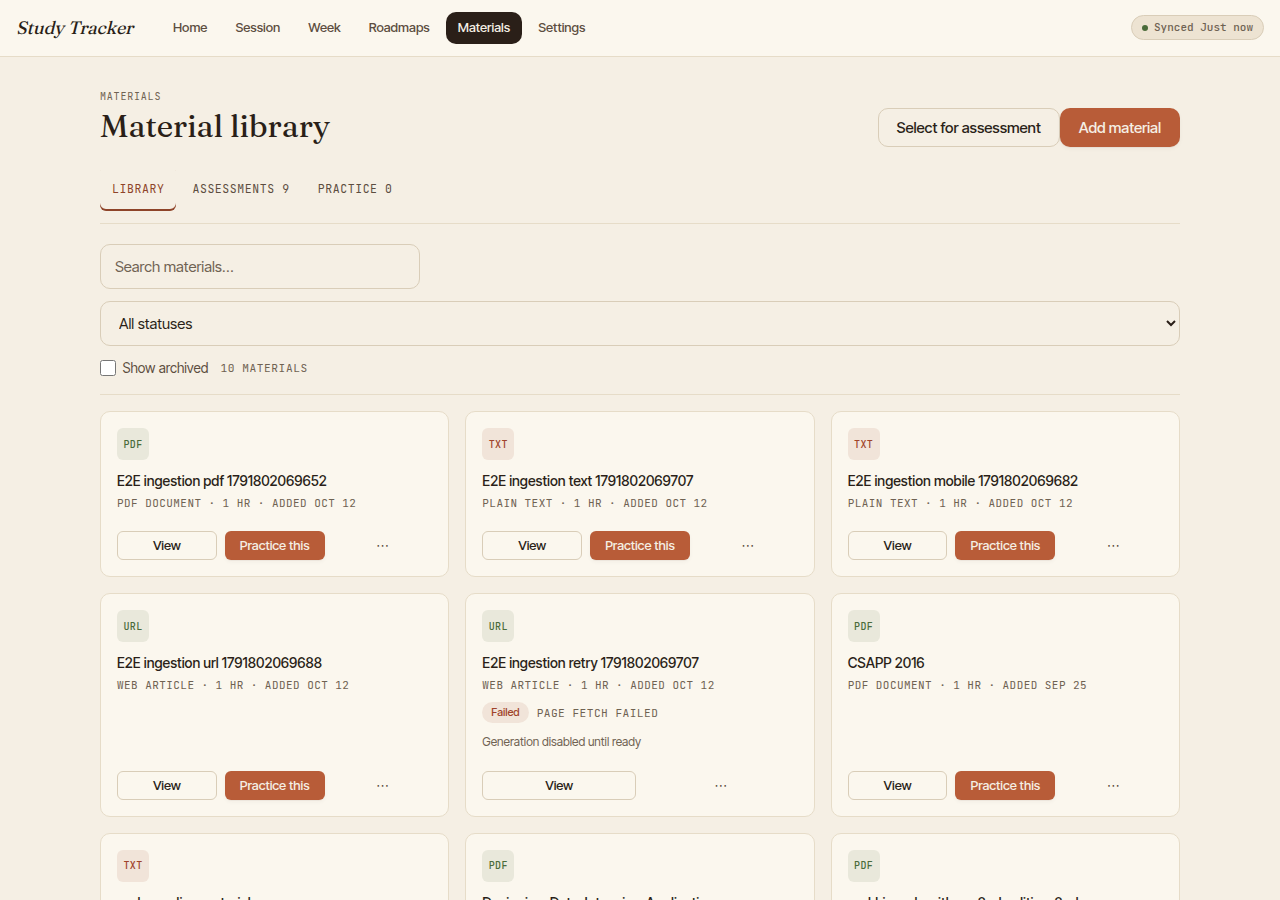
\includegraphics[width=0.85\linewidth, height=0.42\textheight, keepaspectratio]{screenshots/app_materials_library.png}
\caption{The material library: ready cards offer practice while the failed card keeps its badge with a retry action.}
\label{fig:appshot1}
\end{figure}

\subsection{Assessment Generation}
A generation run starts from the config page. The page binds one material, one family, and one scoped chapter before it requests a single question. The server gate admits exactly one family and one question per call. A mixed run alternates families across calls.

The assessment library lists every assessment with its family and status. Cache-first rows paint before revalidation completes. Generation runs as a tracked job. Only a run still marked generating retries in place. A failed run stays failed. Generation adds the second stage to the chain.

\begin{figure}[htbp]
\centering
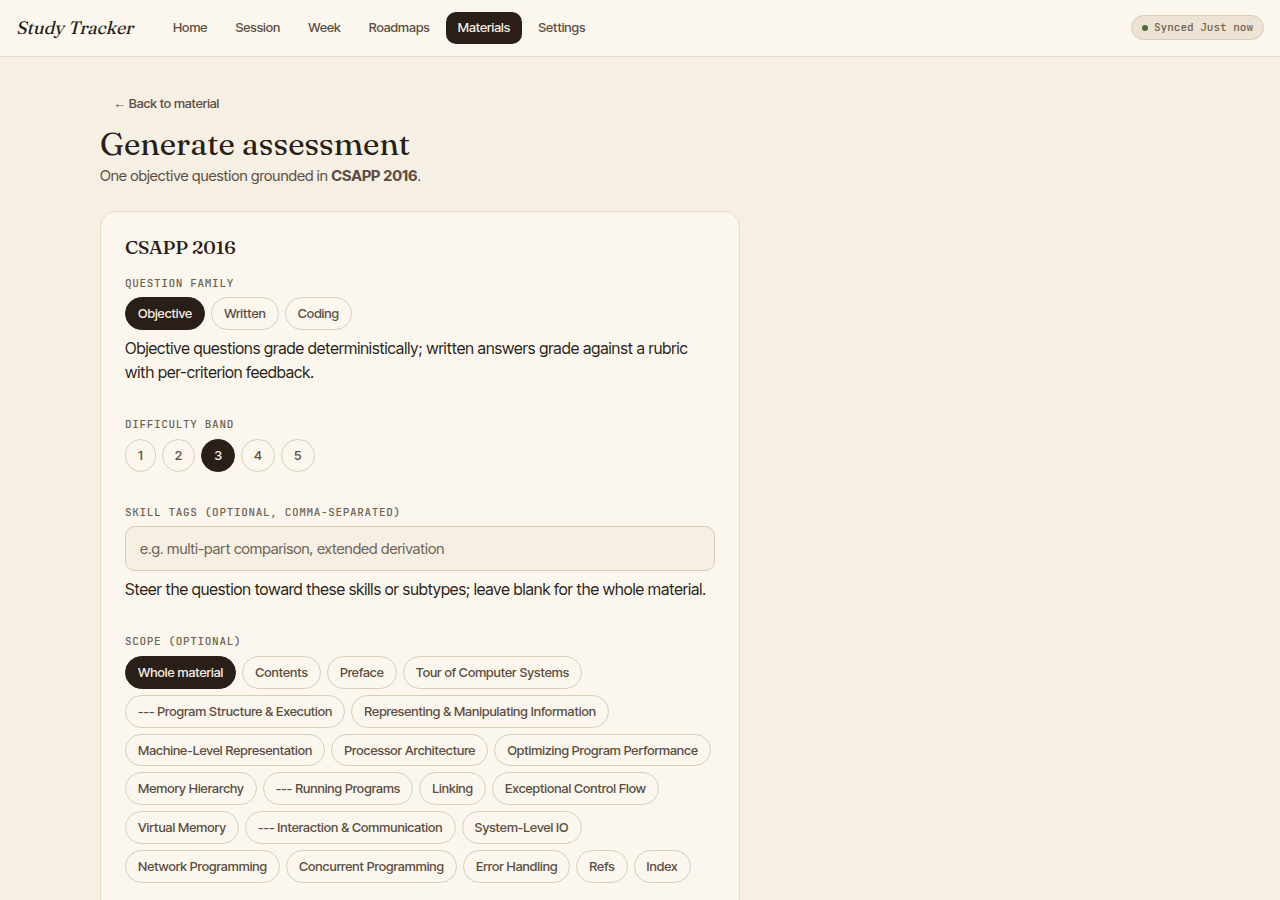
\includegraphics[width=0.85\linewidth, height=0.42\textheight, keepaspectratio]{screenshots/app_assessment_config.png}
\caption{Assessment generation: one material, one family, and one scoped chapter per question.}
\label{fig:appshot2}
\end{figure}

\subsection{Taking and Review}
The taking screens collect one answer per question. They never touch hidden tests, reference solutions, or authored accepted values. Objective answers compare exactly against values authored at generation time. Written answers go to the rubric arm, and coding answers execute against hidden tests. Coding runs in an embedded editor with an advisory client check. The server grade stays final, and no client result enters the record.

The review module shows each attempt beside its grade with per-question detail. Taking and review add the third stage to the chain.

\begin{figure}[htbp]
\centering
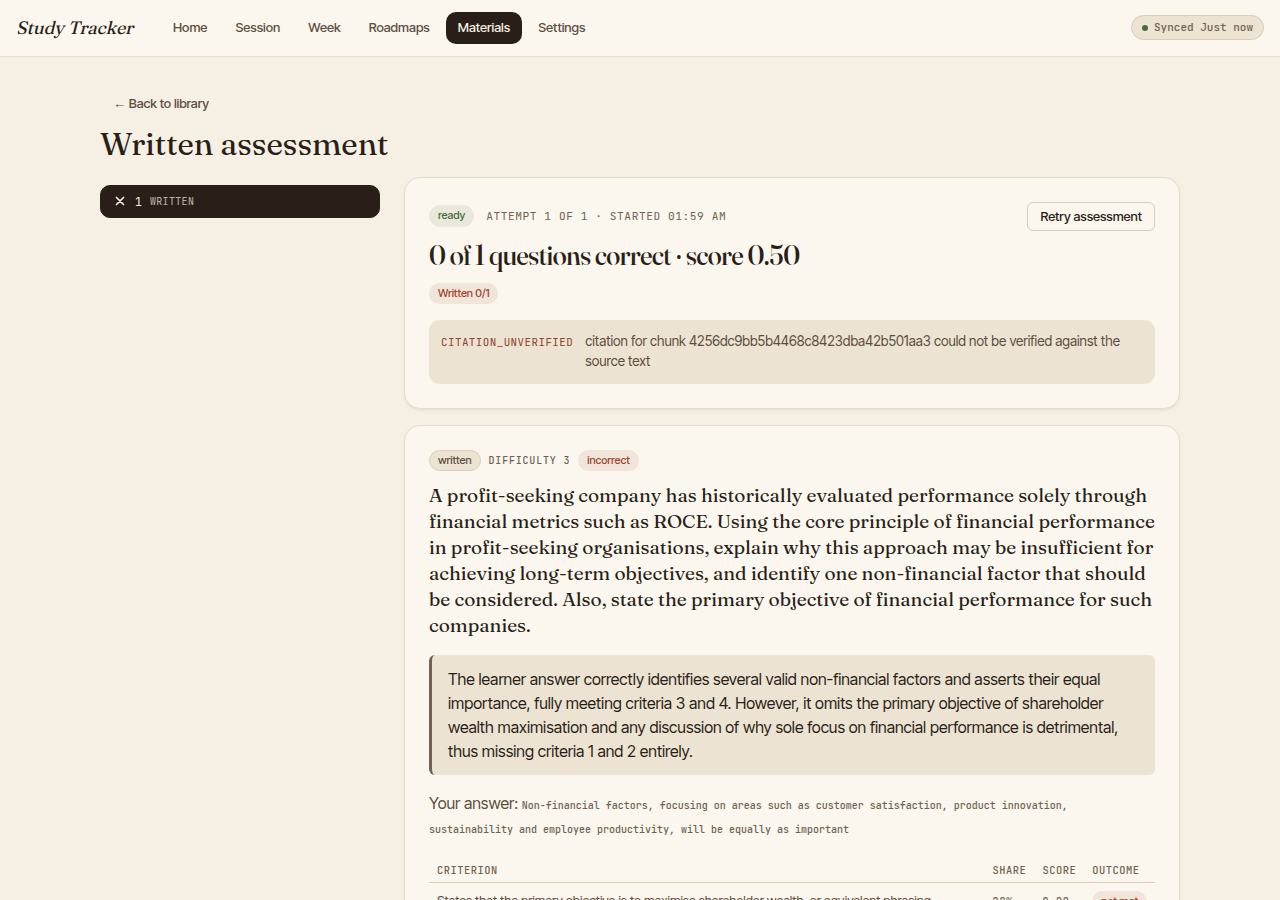
\includegraphics[width=0.85\linewidth, height=0.42\textheight, keepaspectratio]{screenshots/app_assessment_review.png}
\caption{Taking and review: the server grade with per-criterion rubric feedback.}
\label{fig:appshot3}
\end{figure}

\subsection{Practice and Guidance}
The practice hub gathers runs across materials. Each run resolves its questions lazily from the loaded assessments and stores no copies. Pause means leave and return. Neither finish nor abandon invents an observation.

The Socratic coach stays anchored to the page. It streams Nudge, Hint, and Targeted explanation against retrieved chunks and locks Reveal behind an explicit confirmation. The mastery reader beside it shows the current mastery estimate and its advisory, uncalibrated difficulty recommendation (Section~6.1). Practice and guidance add the fourth stage to the chain.

\begin{figure}[htbp]
\centering
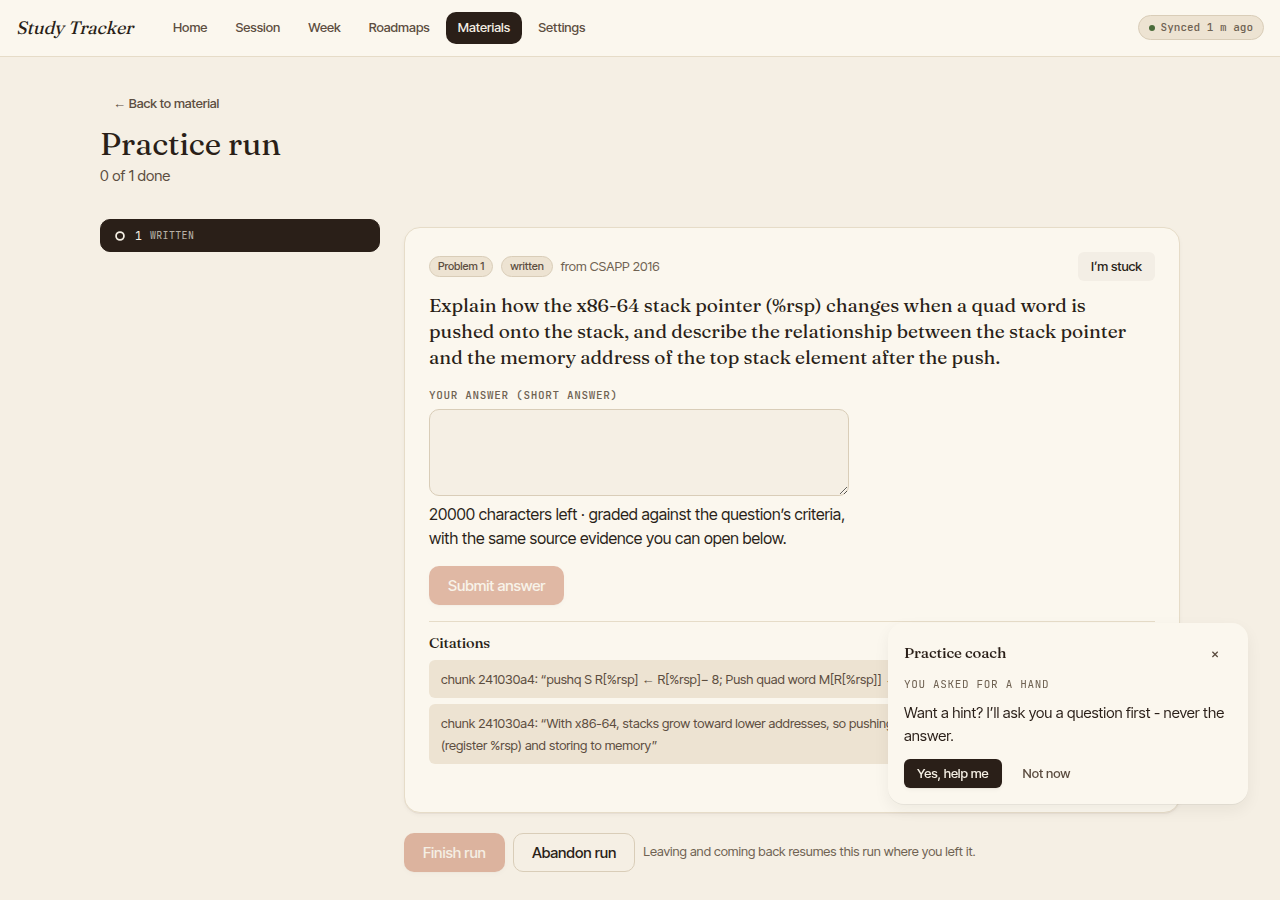
\includegraphics[width=0.85\linewidth, height=0.42\textheight, keepaspectratio]{screenshots/app_practice_run.png}
\caption{Practice run: the lazily resolved question with the Socratic coach anchored to the attempt.}
\label{fig:appshot4}
\end{figure}

\subsection{Feedback and the Closed Loop}
The roadmap detail page carries an evidence ledger. The ledger shows one of four states, cold, updated, stale, or rebuilding, derived from the cached mastery and the latest copy. The feedback-copy endpoint drafts text for updated entries only. The static fallback covers every other state, and the copy never alters a grade.

The loop verdict proposes one choice over the week. Only \texttt{suggest\_replan} passes its verdict pair to the replan screen. Confirming a replan mirrors the pair onto \texttt{RoadmapReplanned} and keeps the plan identity. \texttt{Keep} writes nothing. Figure~\ref{fig:appflow5} shows the complete chain.

\begin{figure}[htbp]
\centering
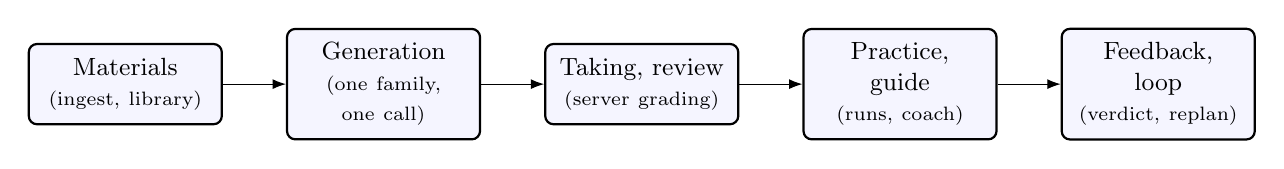
\begin{tikzpicture}[node distance=4mm and 8mm, font=\small, >=Latex,
  a/.style={draw, rounded corners=3pt, line width=0.8pt, align=center, inner sep=5pt, text width=2.1cm, fill=blue!4}]
\node[a] (M) {Materials\\\scriptsize (ingest, library)};
\node[a, right=of M] (G) {Generation\\\scriptsize (one family, one call)};
\node[a, right=of G] (T) {Taking, review\\\scriptsize (server grading)};
\node[a, right=of T] (P) {Practice, guide\\\scriptsize (runs, coach)};
\node[a, right=of P] (F) {Feedback, loop\\\scriptsize (verdict, replan)};
\draw[->] (M) -- (G); \draw[->] (G) -- (T); \draw[->] (T) -- (P); \draw[->] (P) -- (F);
\end{tikzpicture}
\caption{The complete Phase~II application flow: materials reach readiness, generation binds one family per question, taking collects answers under server grading, practice resolves lazily with the coach, and the verdict completes the chain.}
\label{fig:appflow5}
\end{figure}

\begin{figure}[htbp]
\centering
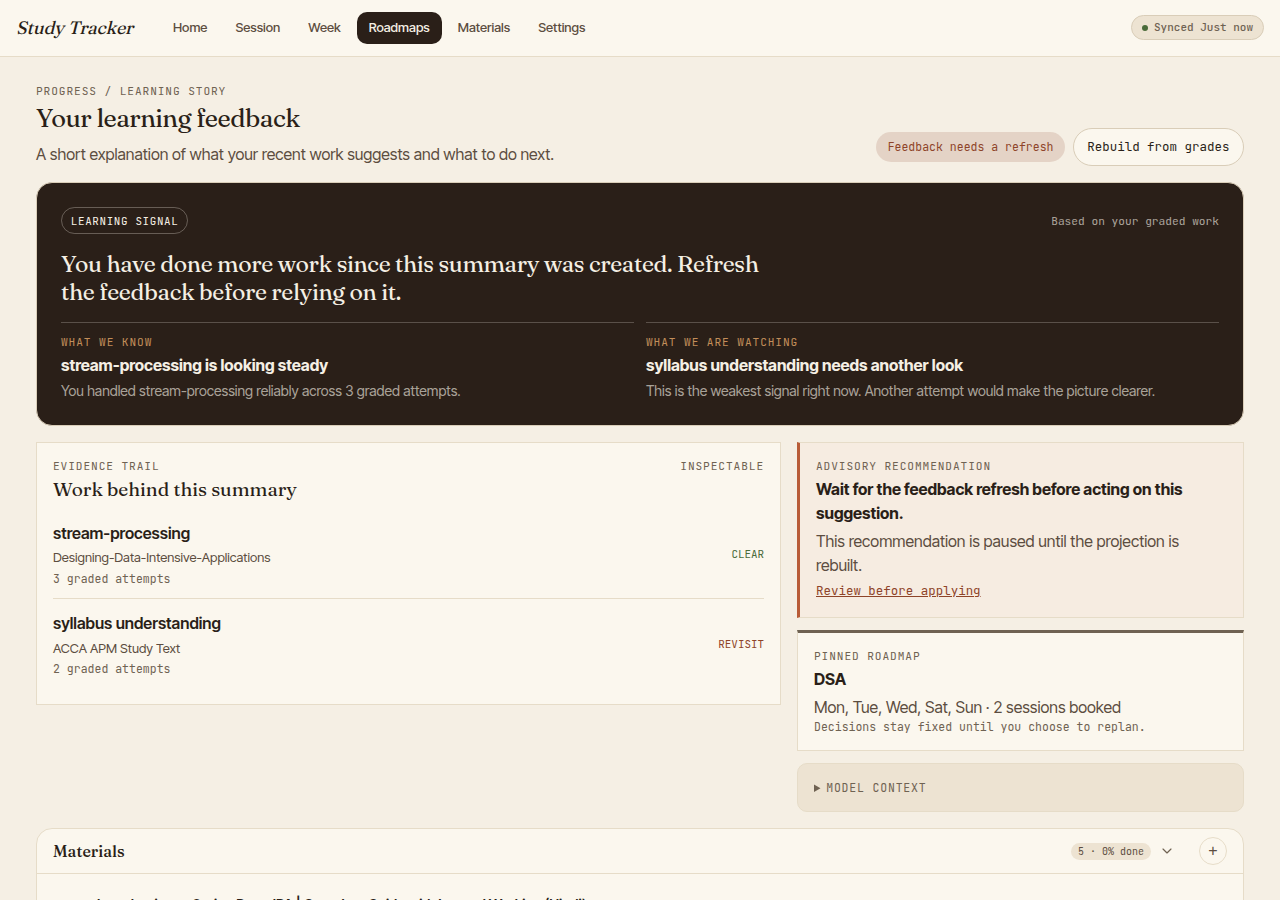
\includegraphics[width=0.85\linewidth, height=0.42\textheight, keepaspectratio]{screenshots/app_roadmap_evidence.png}
\caption{Feedback and the loop: the inspectable evidence trail with the advisory recommendation.}
\label{fig:appshot5}
\end{figure}

These five additions complete the Phase~II application. They are materials and ingestion, assessment generation, taking and review, practice and guidance, and the loop verdict with its replan. Chapter~6 reports the comparison behind them.

\chapter{Results and Discussion}
This chapter reports the offline comparison for each Phase~II loop stage and discusses what the numbers mean for the delivered system. All offline numbers run on the fixed artifacts described in Section~5.2, under the comparison design of Section~4.3. The metrics are those of Table~\ref{tab:phase2-metrics}. This chapter reports against them without redefining them.

Section~6.1 reports generation quality with the retrieval, generation, and tracing tables. Section~6.2 reports live verification as a deployment check. Section~6.3 reports the closed-loop verdict. Section~6.4 reports synthetic longitudinal validation. Section~6.5 discusses the results together.

\section{Generation Quality}
The offline leg scores components against fixed golds behind the fail-closed gate of Figure~\ref{fig:comparison-pipeline}. Three tables carry the leg: retrieval with ranking, generation with its grading signals, and tracing with calibration. Reproducibility for both legs rests on Section~5.4. The harness stays inert unless activated, every call carries one request identifier, and both legs re-run from versioned files.

The harness report and the dated evidence files named in Section~5.4 name the exact inputs. The harness gate verdict for this run is FAIL. The breached gate, \texttt{difficultyMeanAbsBandError}, fires because difficulty calibration is unmeasured (Section~6.1).

Table~\ref{tab:res-retrieval} reports recall and MRR on the coherent 754-chunk ACCA split, the live endpoint row, and the DDIA second corpus. The harness dense and hybrid arms reproduce the recorded in-process baselines exactly, which validates the rerank arm beside them. Reranking lifts hybrid recall at 1 by 7 points (0.60 to 0.67) and recall at 3 by 10 points (0.80 to 0.90). MRR rises by 0.077 (0.720 to 0.797).

The live endpoint reproduces the plain RPC arm exactly (0.60/0.73/0.87/0.703) and its reranked row measures 0.70/0.90/0.93/0.813. The endpoint reranked row sits above the harness arm. The RPC candidate set differs slightly from the in-process copy, so per-question ranks move. The DDIA corpus moves the same direction with larger magnitude. Reranking lifts recall at 1 by 16 points (0.47 to 0.63) and recall at 3 by 17 points (0.73 to 0.90). MRR rises by 0.139 (0.660 to 0.799).

Wilson 95\% intervals on n=30 span about 15 points: harness recall at 1 reads 0.42-0.75 and recall at 3 reads 0.56-0.86. Arm gaps inside that band are descriptive. On the paired endpoint rows the rerank gain is also descriptive. McNemar gives p=0.546 at rank 1 and p=0.131 at rank 3, so neither clears 0.05. No multiplicity correction is applied anywhere in this chapter.

Cross-corpus absolutes are not comparable because the two gold sets were authored independently. Only the arm deltas transfer. The retired 788-split headline (recall at 1 of 0.77, recall at 3 of 0.97, MRR of 0.858) is the frozen-split precedent only. Two rejected arms stay on record: title-prefix indexing shows no gain, and int8 quantization collapses to 0.10 across recalls at 2.45 times speedup.

\begin{table}[htbp]
\centering
\footnotesize
\caption{Retrieval: recall and MRR by arm. ACCA panels share the 30-question harness; the two endpoint rows are the live deployed path (plain RPC plus reranked); DDIA is the second corpus.}
\label{tab:res-retrieval}
\begin{tabular}{l r r r r}
\toprule
\textbf{Corpus and arm} & \textbf{r@1} & \textbf{r@3} & \textbf{r@5} & \textbf{MRR} \\
\midrule
\multicolumn{5}{l}{\textit{ACCA 754-chunk harness}} \\
dense & 0.60 & 0.77 & 0.87 & 0.706 \\
hybrid & 0.60 & 0.80 & 0.87 & 0.720 \\
hybrid\_rerank & 0.67 & 0.90 & 0.93 & 0.797 \\
\midrule
\multicolumn{5}{l}{\textit{Live endpoint, same corpus}} \\
plain (RPC) & 0.60 & 0.73 & 0.87 & 0.703 \\
reranked & 0.70 & 0.90 & 0.93 & 0.813 \\
\midrule
\multicolumn{5}{l}{\textit{DDIA 1094-chunk second corpus}} \\
dense & 0.40 & 0.73 & 0.83 & 0.593 \\
hybrid & 0.47 & 0.73 & 0.83 & 0.660 \\
hybrid\_rerank & 0.63 & 0.90 & 0.97 & 0.799 \\
\bottomrule
\end{tabular}
\end{table}

Generation headlines the delivered reasoning-off arm (S:off, n=30). Schema validity reads 0.9667 (29 of 30) and gold support reads 0.7241 (21 of 29 valid citations). Latency p95 is 10.5~s at cost \$0.00561. Table~\ref{tab:res-generation} carries the six-tier sweep aggregate beside it. The sweep (S-layer, n=180) reads schema validity 0.9611, citation validity 0.9133, gold support 0.7803, near-duplicate rate 0.0044, cost \$0.061289. The generation telemetry behind the sweep counts 361 requests: 281 ok, 37 partial, 35 malformed output, 8 provider errors.

Groundedness measures 0.8667 (26 of 30 judged answerable, Wilson 95\% 0.70-0.95). The 30 judgments cover six distinct questions (S:1 to S:6 with three to six repeats each). The rate describes six clusters rather than 30 independent items. Both the generator and the judge run \texttt{deepseek-v4-flash-0731} with reasoning off. The score is self-judged, and no independent-judge rerun or human audit exists.

The two numbers measure different things. The judge scores whether the cited chunk supports the answer, while gold support scores whether the citation contains the gold string. Schema validity is 0.9611 and citation validity 0.9133, with a near-duplicate rate of 0.0044 at a cost of \$0.061289.

The coding arm refuses material it cannot ground, so derivability on the golds is 0.0 on the pre-top-up run. The fresh live pull derives at 0.5349 over 43 judged attempts (Wilson 95\% 0.39-0.68). Over the full 62 attempts the rate is 0.371 (23 derivable, 20 refusals, 19 failed for other reasons). The rate does not clear the 0.5 gate. The 0.5349 clears it only on the judged pair.

Gold agreement reads 3 of 3. The gold counts are 30 objective, 6 written, and 4 coding (3 derivable plus 1 not), with attempt gate K=5 over 3 fold hashes. The written arm kept its rubric cutoff 0.6 and margin 0.10. The train split favored 0.7, but test agreement fell to 0.5 on a met class of two pairs, so the 0.6 prior shipped.

\begin{table}[htbp]
\centering
\footnotesize
\caption{Generation: delivered S:off arm, S-layer sweep aggregate, groundedness judge, and coding pair. Judge and citation metrics are distinct by construction.}
\label{tab:res-generation}
\begin{tabular}{p{6.4cm} r}
\toprule
\textbf{Metric} & \textbf{Value} \\
\midrule
\multicolumn{2}{l}{\textit{Delivered arm S:off (n=30)}} \\
Schema valid (S:off, 29 of 30) & 0.9667 \\
Gold support (S:off, 21 of 29) & 0.7241 \\
Cost and p95 latency (S:off) & \$0.00561, 10.5~s \\
\midrule
\multicolumn{2}{l}{\textit{Six-tier sweep aggregate (n=180)}} \\
Schema valid & 0.9611 \\
Citation valid & 0.9133 \\
Gold support (citation-contains-gold) & 0.7803 \\
Near-duplicate rate & 0.0044 \\
Cost (USD) & 0.061289 \\
Telemetry (ok, partial, malformed, provider error) & 281, 37, 35, 8 \\
Groundedness, LLM-judged (26 of 30 over six questions) & 0.8667 \\
 Coding derivable on golds (pre-top-up run) & 0.0 \\
Coding derivable live (23 of 43 judged) & 0.5349 \\
Coding derivable live (23 of 62 attempted) & 0.371 \\
\bottomrule
\end{tabular}
\end{table}

Tracing accuracy across three populations sits in Table~\ref{tab:res-bkt}. The bake-off fixed the shipped parameters (p\_init 0.15, p\_learn 0.1, p\_slip 0.05, p\_guess 0.2) at mean AUC 0.785 with ECE 0.057. The live harness over 282 observations across 139 skill sequences gives bkt-v1 AUC 0.7397 with ECE 0.1401 against running-proportion 0.7368 with 0.2679. The external pyBKT accoding anchor reads 0.602 to 0.611 under gate \texttt{masteryMinAuc} 0.6, with ECE 0.272 marked not reportable.

The reading is parity on ranking and a gain on calibration. bkt-v1 matches its baseline on ranking while the calibration error nearly halves on live attempts. The Chapter~4 bake-off pair (0.888 against 0.889) says the same on its cut. The evidence files carry point estimates only, so no interval accompanies AUC or ECE and the parity reading stays descriptive.

Difficulty calibration is recorded as unmeasured. The current pool holds 23 observations on a single question in one band, so the band error is null by construction. The adaptive chip stays uncalibrated-advisory. The update itself is Equation~\ref{eq:bkt-update} with the shipped filter in Listing~\ref{lst:bktforward}.

\begin{table}[htbp]
\centering
\footnotesize
\caption{Knowledge tracing: AUC and calibration across three populations. Parity on ranking; calibration nearly halves on live attempts.}
\label{tab:res-bkt}
\begin{tabular}{l r r}
\toprule
\textbf{Population} & \textbf{AUC} & \textbf{ECE / note} \\
\midrule
Synthetic bake-off (shipped params) & 0.785 & 0.057 \\
Live harness bkt-v1 (282 obs, 139 seqs) & 0.7397 & 0.1401 \\
Live harness running-proportion & 0.7368 & 0.2679 \\
 External pyBKT accoding anchor & 0.602-0.611 & gate 0.6, ECE 0.272 not reportable \\
\bottomrule
\end{tabular}
\end{table}

\section{Live Verification}
The live matrix confirms deployment and never promotes a candidate, per Section~4.3. Objective runs take 2 of 2, written runs grade 4 of 4 with real rubric grades, and coding runs grade 3 of 3. Guide runs pass 2 of 2, practice runs pass 2 of 2, and feedback copy passes 3 of 3. Mastery passes 2 of 2 and review passes 4 of 4. Ingestion passes 5 with 2 skipped.

Every run reports zero console and page errors. AC1, AC3, and AC4 pass with AC2 passing with skips. Each call joins frontend to service logs on one request identifier per Section~5.4.

At scale, the full-book E2E runs through the sidecar. The 572-page fixture (about 23 MB) moves from upload to created at 13.5 s and extracting at 15 s. Embedding takes 48 s and ready takes 101 s. The start-to-ready wall is about 88 s at 10 s poll granularity. The same fixture yields the durable 754-chunk baseline with 0 NULL embeddings. The material was deleted after the run with the card-gone state verified, so the shared account sits as found.

\section{Closed-Loop Decision}
Table~\ref{tab:res-verdict} is this chapter's verdict evidence: the post-fix replay converts 4 of 4 \texttt{suggest\_replan} verdicts into verdict-linked replans. Confidence measures 1.0 with sufficiency from 0.66 to 0.77 across the four archetypes. Every replan extends the deadline and mirrors the exact verdict pair onto \texttt{RoadmapReplanned}. The span runs 32 days for all four from the durable material-scoped \texttt{SessionLogged.payload.date}. The pre-fix contrast is 4 of 4 \texttt{hold} at confidence 0.18 to 0.34 on spanless neutral inputs.

The input fix opened these states: confidence 1.0 would also clear the old 0.9 gate. The gate moved from 0.9 to 0.7. The 0.8 candidate was rejected after a live suggest\_replan sample at 0.79 fell inside the 0.79-0.85 band.

\begin{table}[htbp]
\centering
\footnotesize
\caption{Loop verdict: post-fix replay across four archetypes. Sufficiency 0.66 to 0.77 is the cross-user range; per-archetype decidedAt values sit in the versioned JSON beside the replay evidence.}
\label{tab:res-verdict}
\begin{tabular}{l l r r l l}
\toprule
\textbf{Archetype} & \textbf{Verdict} & \textbf{Conf} & \textbf{Suff} & \textbf{Option} & \textbf{Converted} \\
\midrule
steady & suggest\_replan & 1.0 & 0.66-0.77 & extend-deadline & yes \\
crammer & suggest\_replan & 1.0 & 0.66-0.77 & extend-deadline & yes \\
struggling & suggest\_replan & 1.0 & 0.66-0.77 & extend-deadline & yes \\
returning & suggest\_replan & 1.0 & 0.66-0.77 & extend-deadline & yes \\
\bottomrule
\end{tabular}
\end{table}

\section{Synthetic Longitudinal Validation}
The longitudinal leg replays four synthetic archetypes with known posture: steady, crammer, struggling, and returning. Development histories stay separate from evaluation histories, so a conversion reflects behavior instead of fitting. The 24-cell adherence emission and the per-archetype decidedAt values sit in Appendix~\ref{ch:appendix}. Twenty weekly values are observed. Week 5 is not observed for any user. This section reports the headline with its caveat.

Next-week adherence is not observed for any of the four in the post-replan extension week. Capture ran one day before the deadline, so no post-replan sessions could be logged. The 0.000 in Table~\ref{tab:app-adherence} marks an unobserved week, not a measured zero and not a learning result.

The 12 mastery rows sit at about 0.1067 throughout after the replay, below the prior of 0.15 by construction. The seeded scripts answer about 90 percent wrong because they prioritize grading-path coverage over learner success. Those rows measure the scripts and are never cited as tracing validation. The tracing evidence lives in Table~\ref{tab:res-bkt}.

Each of the 4 verdicts joins its \texttt{RoadmapReplanned} by the exact verdict pair with createdAt at or after decidedAt. A seed-shape finding is recorded with the evidence. The seed writes one timestamp with a zone offset while the booking reference uses milliseconds. The strict-equality join silently mistraces until emission canonicalizes the instant. The seed-shape defect was recorded with the evidence. No product code changed.

The dip-window replay pins the browser clock to the week-3 trough for every archetype. All four hold at confidence 0.28 to 0.35 with sufficiency 0.66 to 0.77 and convert nothing, because \texttt{Keep} writes nothing. A September-12 pin for the struggling archetype flips the choice to \texttt{suggest\_replan} at 0.61 to 0.69 but the gate holds it. The gradient matches the design: trough holds on the merits, week 4 proposes below the gate, and the rebound eve converts at 1.0.

The replay drove verdicts only and produced no new graded attempts, so the difficulty pool is unchanged. Cloud replan counts stayed at the recorded per-user values (crammer 1, returning 2, steady 1, struggling 2), with no cloud history rewritten. Four caveats travel with this leg. The clock pins to 2026-10-14, and capture covers the rebound era rather than the week-3 dip. The onboarding gate is local only, and cold restore duplicates locally while extracting from cloud only.

\section{Discussion}
Read together, the results move the loop from logged time to graded evidence. Tracing holds ranking parity while the calibration error nearly halves on live attempts, because the per-skill updater tracks the graded attempts the baseline averages away. Reranking lifts recall on both corpora, with the larger DDIA gain coming from the noisier candidate set. Coding refuses ungroundable material instead of inventing a question, and the live pull clears the 0.5 gate only on the judged pair.

Difficulty calibration is unmeasured because the pool holds one question in one band. Next-week adherence is unobserved because capture ran one day before the deadline. Two results are comparative gains: retrieval ranking and the 4 of 4 verdict conversion with its pre-fix contrast. Two are descriptive: grounded generation at 0.8667 with near-duplicates at 0.0044, and the full-book path reaching ready in about 88 s.

One refinement stays validated but unshipped from Phase~I: the split-conformal interval correction. It does not enter the delivered behavior and returns in Chapter~7 as future work.

Transfer holds in the sense the design needs. Dense and hybrid reproduce their baselines exactly on the rerun, which validates the rerank arm. The DDIA corpus repeats the ACCA direction at larger magnitude.

The scope is a single learner with synthetic histories in place of a classroom study. No fixed-plan control arm ran, so the 4-of-4 conversion has no efficacy comparison. One difficulty question is eligible, with the four replay caveats of Section~6.4. Figure~\ref{fig:architecture} shows where each stage from Table~\ref{tab:method-candidates} now runs.

\section{Threats to Validity}
Construct validity is limited on two fronts. The groundedness score is self-judged: the generator and the judge share the same model with reasoning off, and no independent judge or human audit exists. The longitudinal scripts prioritize grading-path coverage over learner success and answer about 90 percent wrong, so the mastery rows measure the scripts rather than tracing.

Internal validity rests on synthetic histories with no fixed-plan control, so the verdict conversion cannot claim efficacy on learning. Week 5 is unobserved rather than measured. The 0.5 coding gate clears only on the judged pair. The full-denominator rate of 0.371 does not clear it. The harness gate verdict for this run is FAIL on the unmeasured difficulty band.

External validity is narrow: one learner, one frozen ACCA textbook split plus the DDIA second corpus, and pinned model versions with no drift monitoring. Retrieval and generation numbers need not transfer to other materials or models.

An ethics and security paragraph travels with these limits. Learner material sent to OpenRouter for generation, grading, and judging travels to a third party, and the report states no retention or redaction contract. A classroom deployment must add one. Piston executes hidden tests server-side through the profile on port~2000, but the report states no resource or egress bound for that sandbox. Adversarial material that injects instructions into generation or grading is untested. No learner usability evidence exists: every live check is a deployment pass by the developer.

\section{Summary}
Read together, the results validate the integration rather than the learning. Reranking lifts recall on both corpora, but the paired test cannot separate the gain from noise at n=30. The delivered S:off arm generates valid questions cheaply, and groundedness reads 0.8667 over six self-judged clusters. Coding clears its gate only on the judged pair. Tracing holds ranking parity while nearly halving calibration error.

The loop converts 4 of 4 verdicts into verdict-linked replans with no fixed-plan control, and next-week adherence is unobserved. The system is a working integration of graded evidence into planning, with efficacy on learning deferred.

\chapter{Conclusion and Future Work}
This chapter closes the report. Section~7.1 concludes what the two phases delivered. Section~7.2 sets out future work.
% Drafting starts here (grill pending).


% ---- Appendix (supplementary Ch6 tables/figures; Q7a shell) ----
\appendix
\chapter{Supplementary Tables and Figures}
\label{ch:appendix}
This appendix collects the supplementary tables and figures referenced from Chapter~6. Each item repeats its in-text number so the reader can move between the discussion and the full table without searching.
% Supplementary Ch6 tables and figures land here during drafting (Q7a shell).


\newpage
% ---- Bibliography (kept in main; Pillar-A then Pillar-B) ----
\addcontentsline{toc}{chapter}{Bibliography}
\begin{thebibliography}{99}
% Entries in first-citation order (Ch1-Ch2). Pillar-B entries under the separator.
% Metadata verified 2026-10-23 (Batch 2): titles, venues, volumes, pages, DOIs checked against publisher records.

\bibitem{chen2024} Chen, A. M., Palacci, A., V\'elez, N., Hawkins, R. D., Gershman, S. J., ``A Hierarchical Bayesian Model of Adaptive Teaching,'' \textit{Cognitive Science}, vol. 48, no. 7, Art. e13477, 2024, doi:10.1111/cogs.13477.

\bibitem{alhazbi2024} Alhazbi, S., et al., ``Using Learning Analytics to Measure Self-Regulated Learning: A Systematic Review,'' \textit{Journal of Computer Assisted Learning}, vol. 40, no. 4, pp. 1658--1674, 2024, doi:10.1111/jcal.12982.

\bibitem{islam2024} Islam, M., et al., ``Predict Students' Performance and Optimize Preparatory Leave,'' \textit{Proc. 27th Int. Conf. on Computer and Information Technology (ICCIT)}, IEEE, pp. 728--733, 2024, doi:10.1109/iccit64611.2024.11021881.

\bibitem{zanellati2024} Zanellati, A., Di Mitri, D., Gabbrielli, M., Levrini, O., ``Hybrid Models for Knowledge Tracing: A Systematic Review,'' \textit{IEEE Transactions on Learning Technologies}, vol. 17, pp. 1021--1036, 2024.

\bibitem{mai2025} Mai, N.~T., Cao, W., Liu, W., ``Interpretable Knowledge Tracing via Transformer--Bayesian Hybrid Networks,'' \textit{Applied Sciences}, vol. 15, Art. 9605, 2025, doi:10.3390/app15179605.

% --- Pillar-B references (Phase II) ---
\bibitem{itemgen2024} Chan, K. W., et al., ``Automatic Item Generation in Various STEM Subjects Using Large Language Model Prompting,'' \textit{Computers and Education: Artificial Intelligence}, vol. 8, Art. 100344, 2024, doi:10.1016/j.caeai.2024.100344.

\bibitem{lecturequiz2026} Shintani, S. A., ``Self-hosted Lecture-to-Quiz: Local LLM MCQ Generation with Deterministic Quality Control,'' arXiv:2603.08729 [cs.CY], 2026 (unrefereed preprint).

\bibitem{kctag2024} Moore, S., Schmucker, R., Mitchell, T., Stamper, J., ``Automated Generation and Tagging of Knowledge Components from Multiple-Choice Questions,'' \textit{Proc. 11th ACM Conf. on Learning @ Scale (L@S '24)}, Atlanta, GA, USA, 2024, doi:10.1145/3657604.3662030.

\bibitem{llmgrade2024} Ta, N. B. D., Chai, Y. M., ``Automatic Grading of Short Answers Using Large Language Models in Software Engineering Courses,'' \textit{Proc. 2024 IEEE Global Engineering Education Conf. (EDUCON)}, Kos Island, Greece, pp. 1--10, 2024, doi:10.1109/educon60312.2024.10578839.

\bibitem{uzun2025} Uzun, Y., Suraworachet, W., Zhou, Q., Gauthier, A., Cukurova, M., ``Engagement with Analytics Feedback and Its Relationship to Self-Regulated Learning Competence and Course Performance,'' \textit{International Journal of Educational Technology in Higher Education}, vol. 22, Art. 17, 2025, doi:10.1186/s41239-025-00515-3.

\bibitem{gaming2026} Zhang, J., et al., ``Understanding Gaming the System by Analyzing Self-Regulated Learning in Think-Aloud Protocols,'' \textit{Proc. 16th Int. Learning Analytics and Knowledge Conf. (LAK)}, ACM, 2026, doi:10.1145/3785022.3785025.

% --- Batch-4 records (verified 2026-10-23 against publisher, ACM, ACL, and Scholar-indexed records) ---
\bibitem{corbett1995} Corbett, A. T., Anderson, J. R., ``Knowledge Tracing: Modeling the Acquisition of Procedural Knowledge,'' \textit{User Modeling and User-Adapted Interaction}, vol. 4, pp. 253--278, 1995, doi:10.1007/BF01099821.

\bibitem{page1954} Page, E. S., ``Continuous Inspection Schemes,'' \textit{Biometrika}, vol. 41, no. 1/2, pp. 100--115, 1954, doi:10.1093/biomet/41.1-2.100.

\bibitem{rasmussen2006} Rasmussen, C. E., Williams, C. K. I., \textit{Gaussian Processes for Machine Learning}, MIT Press, 2006.

\bibitem{vovk2005} Vovk, V., Gammerman, A., Shafer, G., \textit{Algorithmic Learning in a Random World}, Springer, 2005.

\bibitem{vanlehn2011} VanLehn, K., ``The Relative Effectiveness of Human Tutoring, Intelligent Tutoring Systems, and Other Tutoring Systems,'' \textit{Educational Psychologist}, vol. 46, no. 4, pp. 197--221, 2011, doi:10.1080/00461520.2011.611369.

\bibitem{koedinger2007} Koedinger, K. R., Aleven, V., ``Exploring the Assistance Dilemma in Experiments with Cognitive Tutors,'' \textit{Educational Psychology Review}, vol. 19, no. 3, pp. 239--264, 2007, doi:10.1007/s10648-007-9049-0.

\bibitem{anderson1995} Anderson, J. R., Corbett, A. T., Koedinger, K. R., Pelletier, R., ``Cognitive Tutors: Lessons Learned,'' \textit{Journal of the Learning Sciences}, vol. 4, no. 2, pp. 167--207, 1995, doi:10.1207/s15327809jls0402\_2.

\bibitem{cepeda2006} Cepeda, N. J., Pashler, H., Vul, E., Wixted, J. T., Rohrer, D., ``Distributed Practice in Verbal Recall Tasks: A Review and Quantitative Synthesis,'' \textit{Psychological Bulletin}, vol. 132, no. 3, pp. 354--380, 2006, doi:10.1037/0033-2909.132.3.354.

\bibitem{settles2016} Settles, B., Meeder, B., ``A Trainable Spaced Repetition Model for Language Learning,'' \textit{Proc. 54th Annual Meeting of the Association for Computational Linguistics (Vol. 1: Long Papers)}, pp. 1848--1858, 2016, doi:10.18653/v1/P16-1174.

\bibitem{zheng2023} Zheng, L., et al., ``Judging LLM-as-a-Judge with MT-Bench and Chatbot Arena,'' \textit{Advances in Neural Information Processing Systems 36 (Datasets and Benchmarks Track)}, pp. 46595--46623, 2023.

\bibitem{embretson2000} Embretson, S. E., Reise, S. P., \textit{Item Response Theory for Psychologists}, Erlbaum, 2000.

\bibitem{hattie2007} Hattie, J., Timperley, H., ``The Power of Feedback,'' \textit{Review of Educational Research}, vol. 77, no. 1, pp. 81--112, 2007, doi:10.3102/003465430298487.

\bibitem{chi2014} Chi, M. T. H., Wylie, R., ``The ICAP Framework: Linking Cognitive Engagement to Active Learning Outcomes,'' \textit{Educational Psychologist}, vol. 49, no. 4, pp. 219--243, 2014, doi:10.1080/00461520.2014.965823.

\bibitem{piech2015} Piech, C., et al., ``Deep Knowledge Tracing,'' \textit{Advances in Neural Information Processing Systems 28}, 2015, arXiv:1506.05908.

\bibitem{niculescu2005} Niculescu-Mizil, A., Caruana, R., ``Predicting Good Probabilities with Supervised Learning,'' \textit{Proc. 22nd Int. Conf. on Machine Learning (ICML)}, pp. 625--632, 2005, doi:10.1145/1102351.1102464.

\bibitem{bloom1984} Bloom, B. S., ``The 2 Sigma Problem: The Search for Methods of Group Instruction as Effective as One-to-One Tutoring,'' \textit{Educational Researcher}, vol. 13, no. 6, pp. 4--16, 1984, doi:10.3102/0013189X013006004.

\bibitem{shute2008} Shute, V. J., ``Focus on Formative Feedback,'' \textit{Review of Educational Research}, vol. 78, no. 1, pp. 153--189, 2008, doi:10.3102/0034654307313407.

\bibitem{roediger2006} Roediger, H. L., Karpicke, J. D., ``Test-Enhanced Learning: Taking Memory Tests Improves Long-Term Retention,'' \textit{Psychological Science}, vol. 17, no. 4, pp. 249--255, 2006, doi:10.1111/j.1467-9280.2006.01693.x.

\bibitem{dunlosky2013} Dunlosky, J., et al., ``Improving Students' Learning with Effective Learning Techniques: Promising Directions from Cognitive and Educational Psychology,'' \textit{Psychological Science in the Public Interest}, vol. 14, no. 1, pp. 4--58, 2013, doi:10.1177/1529100612453266.

\bibitem{kasneci2023} Kasneci, E., et al., ``ChatGPT for Good? On Opportunities and Challenges of Large Language Models for Education,'' \textit{Learning and Individual Differences}, vol. 103, Art. 102274, 2023, doi:10.1016/j.lindif.2023.102274.

\end{thebibliography}
\end{document}
